\section{Ablations}\label{sec:ablation}
\GenAblationTable
\paragraph{Loss terms.} Table~\ref{tab:ablation} (upper block) varies the training objective on MNIST.
\begin{itemize}
\item \textbf{Percept-similarity term is essential.} Without it, training collapsed within the first 300 steps to currents below the rheobase, i.e.\ no phosphenes. The result is SSIM \AbNoPerSsim\ and accuracy \AbNoPerAcc, with a charge of essentially zero. With the decoder loss as the only objective, the gradient reaching a dark electrode passes through the sub-rheobase ReLU and the narrow threshold surrogate. Once most electrodes fall below threshold, that gradient vanishes.
\item \textbf{Decoder loss did not help at this scale.} Dropping it gave SSIM \AbNoRecSsim\ and accuracy \AbNoRecAcc, against \AbMainSsim\ and \AbMainAcc\ for the full objective.
\item \textbf{Charge cost is cheap.} Removing it raised summed charge from \AbMainCharge\ to \AbNoChgCharge\,\textmu C per phase without improving fidelity (SSIM \AbNoChgSsim).
\end{itemize}

\paragraph{Safety limits.} Removing the active-electrode cap and the charge cost, and raising the ceiling to 200\,\textmu A, gives better images: SSIM \AbUnconSsim\ against \AbMainSsim. The price is \AbUnconActive\ active electrodes instead of \AbMainActive\ and \AbUnconCharge\ against \AbMainCharge\,\textmu C of charge per phase, while recognition is unchanged (\AbUnconAcc\ against \AbMainAcc). For a device that must manage charge, heat and power, the constrained operating point is clearly preferable.

\paragraph{Electrode count and layout.} The lower block of Table~\ref{tab:ablation} and Fig.~\ref{fig:ablation} vary the implant.
\begin{itemize}
\item \textbf{Threads.} With 64 and 256 sites the learned encoder still beats intensity sampling on recognition: \AbThrAAcc\ against \AbThrAIntAcc, and \AbThrBAcc\ against \AbThrBIntAcc. Its relative advantage is largest when phosphenes are scarce.
\item \textbf{One Utah array (96 channels).} It covers only a $\sim$0.6$^\circ$ patch near $2^\circ$ eccentricity, so neither encoder can convey digits (accuracy \AbUtahAAcc\ learned, \AbUtahAIntAcc\ intensity). End-to-end training here also collapsed to no stimulation: the charge fell to essentially zero within 300 steps, the same dead-zone failure as above.
\item \textbf{Sixteen Utah arrays (1024 contacts).} They reach \AbUtahBAcc\ (learned) and \AbUtahBIntAcc\ (intensity); here intensity sampling is slightly better. Both are well below the same number of thread sites (\AbMainAcc), because the contacts cluster into 16 small patches of the visual field, where neighbouring phosphenes overlap.
\end{itemize}

\begin{figure}[t]
\centering
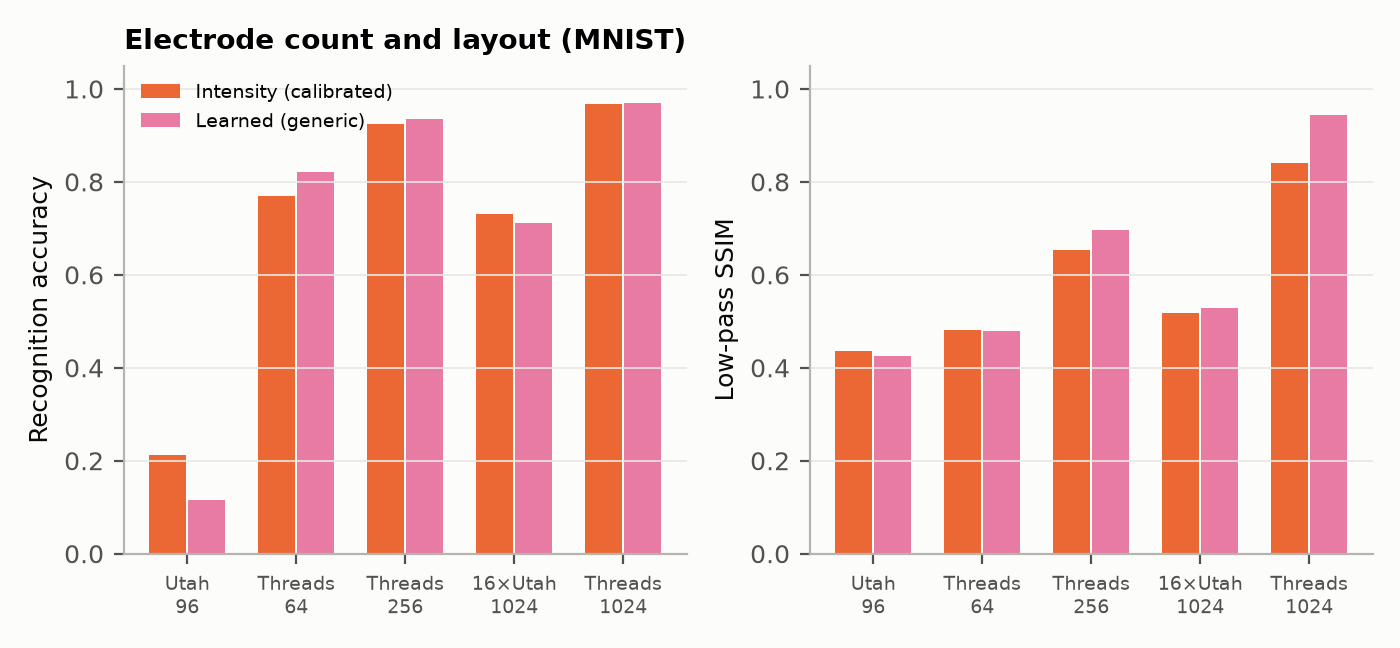
\includegraphics[width=\columnwidth]{fig_ablation_layouts.png}\\[2pt]
\IfFileExists{../results/figures/fig_adaptation_shots.png}{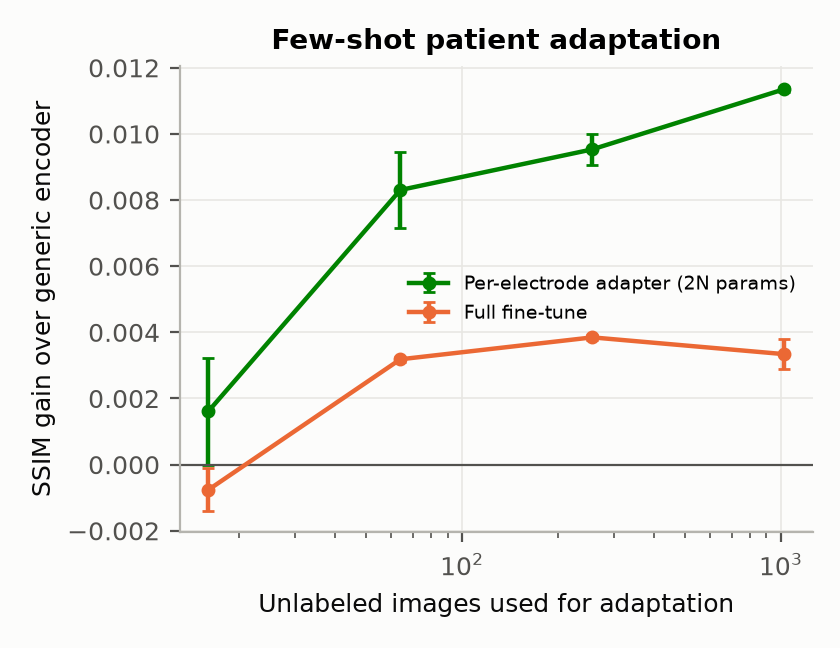
\includegraphics[width=0.75\columnwidth]{fig_adaptation_shots.png}}{}
\caption{\textbf{Top:} recognition and low-pass SSIM against electrode layout (MNIST, seed 0), learned encoder against intensity sampling. \textbf{Bottom:} SSIM gain from patient adaptation against the number of unlabeled images. MNIST, two held-out patients, 150 steps. With 64 or more images, adapter-only fine-tuning (2$N$ parameters) gains more than full fine-tuning.}
\label{fig:ablation}\label{fig:adapt}
\end{figure}


\section{Discussion}
\paragraph{What the learned encoder learns.} Three observations follow from Fig.~\ref{fig:examples} and from the budget diagnostics (\texttt{results/eval/diagnostics.json}):
\begin{itemize}
\item \textbf{Budget allocation.} Intensity sampling fills its 25\% active-electrode budget with whichever sites are brightest, and can drop whole parts of a shape (the ``W''). The learned encoder activates fewer sites (\NumMnistLearnActive\ against \NumMnistIntActive\ on MNIST) but keeps strokes continuous.
\item \textbf{Thresholds.} The generic encoder does not know the patient's thresholds, and \NumMnistLearnSupraPct--\NumCifarLearnSupraPct\% of its delivered currents exceed them (MNIST to CIFAR). The calibrated baseline reaches \NumMnistIntSupraPct\% on MNIST. Wasted sub-threshold stimulation is therefore a remaining inefficiency that a threshold-aware adapter or a threshold input channel could remove.
\item \textbf{Natural images.} With only $\sim$250 phosphenes the learned encoder renders coarse luminance layout and large contours rather than texture, which resembles a learned scene simplification. This is where low-pass SSIM rises most (\NumCifarIntLp\ to \NumCifarAdaptLp).
\end{itemize}

\paragraph{Why a retinotopic read-out.} A dense output layer for 1024 electrodes would hold most of the model's parameters, would be tied to one electrode layout, and could not use the fact that nearby phosphenes should get similar commands. Our convolutional map with a bilinear read-out avoids all three problems:
\begin{itemize}
\item it has \NumEncParams\ parameters in total;
\item the read-out positions are a buffer, not learned weights, so the trunk is not tied to one layout (we did not test transfer between layouts);
\item all per-person variation sits in a 2$N$-parameter adapter.
\end{itemize}
This split fits the clinical workflow. A generic model is trained once in simulation. Each patient's adapter is then fitted to that person's mapping data: thresholds and dead electrodes now, phosphene locations once mapped. If no calibrated forward model is available, the adapter's low dimension makes it a natural target for preference-based optimisation \citep{granley2023human}.

\paragraph{Implications for implant design.} The layout ablation separates electrode \emph{count} from \emph{coverage}. One Utah array covers \NumCovUtahNine\% of the central field, so neither encoder conveys digits with it (accuracy at most \AbUtahAIntAcc). Sixteen arrays with 1024 contacts cover \NumCovUtahThou\%, because each 3\,mm array lands on one small patch of the field. The same number of independently placed thread sites covers \NumCovThrThou\%. Under our assumptions, a 1024-channel device gains most from spreading its insertion sites over the reachable cortex. Packing more contacts into rigid grids helps far less.

\section{Limitations}\label{sec:limits}
\begin{itemize}
\item \textbf{Simulation only.} Every result depends on the phosphene model. That model is fitted to one human Utah-array study \citep{fernandez2021visual}, a few earlier reports, and parameters some of which the dynaphos authors describe as not fitted to data (e.g.\ $\tau_{\mathrm{act}}$).
  \begin{itemize}
  \item Our threshold distribution has mean \NumThrMean\,\textmu A, lower than the 66.8\,\textmu A reported by Fernández et al.
  \item The model leaves out phosphene shape, colour and flicker; interactions between electrodes (current summation, threshold reduction under simultaneous stimulation, which Fernández et al.\ observed); and gaze-contingent shifts of phosphene location.
  \end{itemize}
\item \textbf{Planar cortex.} The thread layout assumes uniformly reachable V1 on a plane. Much of real V1 lies inside the calcarine sulcus, so coverage is optimistic. The layout is our idealisation, not a device specification.
\item \textbf{Static frames.} We optimise single 166\,ms frames. Temporal encoding (dynamic current steering, \citealp{beauchamp2020dynamic}) and managing habituation over seconds are not addressed, although the simulator models habituation.
\item \textbf{Recognition proxy.} A CNN trained on percepts upper-bounds what a person could learn: it has unlimited training, no attention limits and no fatigue. Human psychophysics with simulated prosthetic vision would be the next validation step.
\item \textbf{Scale.} Networks are small, data are low-resolution benchmarks, training is 1500 steps, and patients are few. Standard deviations over three seeds are small, but conclusions about natural scenes (CIFAR) in particular are preliminary.
\item \textbf{Two training failures.}
  \begin{itemize}
  \item With a single 96-channel array, end-to-end training collapsed to no stimulation (discussed above).
  \item Without safety limits, a first run that initialised every electrode at 100\,\textmu A also collapsed. Its training log (\texttt{results/extra\_runs/}) shows the charge term going to zero. The reported unconstrained variant starts at 50\,\textmu A like every other run.
  \end{itemize}
  Both point to dead zones (sub-rheobase currents and saturated sigmoids) as a practical pitfall of end-to-end stimulation learning.
\end{itemize}

\section{Broader impact and safety}
The stimulus encoder is the software that decides how much current enters a person's brain, so it is safety-critical. Our design keeps safety outside the learned component:
\begin{itemize}
\item the same hard clamp and active-electrode cap apply to every encoder, learned or not;
\item the learned model can only choose \emph{within} the safe set.
\end{itemize}
A deployable system would also need charge-density limits specific to the electrode material and geometry \citep{shannon1992model,cogan2008neural}, limits on cumulative charge over time, monitoring for threshold drift, and clinician-set per-electrode ceilings. Our numbers are not a statement about any real device's safety.

Simulated recognition rates must not be read as predictions of what a blind person will see. Communicating that uncertainty honestly matters, because expectations for these devices are high. This is an independent project, not affiliated with or endorsed by Neuralink, and it uses no proprietary data.

\section{Reproducing at full scale}\label{sec:repro}
Everything above comes from \texttt{scripts/run\_cpu.sh} (\texttt{configs/cpu.yaml}). That script runs the pipeline end to end: data, simulator validation, training, evaluation, ablations, adaptation, figures and website export, followed by the unit tests.

\texttt{scripts/run\_gpu.sh} runs the same code with \texttt{configs/gpu.yaml} on a CUDA machine. The device is detected automatically; the CNNs run under bfloat16 autocast and the simulator in float32. It scales up:
\begin{itemize}
\item training: 20k steps at batch size 128, 100k training images, network width 48;
\item seeds and patients: five seeds, 64 training patients, ten test patients;
\item evaluation: 50k classifier images, 300-step per-image optimisation, three ablation seeds, and a 2048-site layout.
\end{itemize}
The script creates its own virtual environment from \texttt{requirements-gpu.txt} and downloads the datasets. The figures, \texttt{metrics.json} and these tables are regenerated from its outputs by \texttt{paper/make\_tables.py}.
